\section{Theory}
\label{sec:theory}

Towards developing a constant space HPYP model and inference procedure we first review dependent PY processes in Section~\ref{sec:dpyp}.  We then develop a dependent HPYP in Section~\ref{sec:dhpyp}. In both of these processes dependency arises from operations on customers in the CRP representation. We define our dependent HPYP in terms of operations on restaurants.

%While the SM model demonstrates promising empirical results \cite{Gasthaus} we are unsatisfied with the linear space requirement for reasons stated earlier.  We propose a framework for limiting the memory required to represent models based on the hierarchical Pitman-Yor process.  Estimation in this framework can be viewed either as a valid inference scheme for a model based on a dependent set of hierarchical Pitman-Yor processes or as an approximate inference technique for a non-varying model.

\subsection{Dependent Pitman-Yor process} 
\label{sec:dpyp}

The $\ES_N(d,c)$ distribution discussed in Section~\ref{basicModel} has an important consistency property. In the Chinese restaurant metaphor this consistency property corresponds to the fact that if a customer is removed uniformly at random, the remaining customer configuration represents a partition of the first $N-1$ integers following the $\ES_{N-1}(d,c)$ distribution \cite{Pitman1995}.  This removal of a customer is known as a deletion operation.  Another deletion operation, known as size-biased deletion, is one in which a customer is chosen uniformly at random and all customers seated at the same table are removed from the restaurant. Size biased deletion is known to satisfy a consistency property for the one parameter Ewen's distribution \cite{Kingman1978}, but the same is not true for the two parameter case \cite{Pitman1995}.

This consistency property is exploited in a generative procedure defined in the restaurant representation to draw samples  $\{ \{ \theta_j^t \}_{j = 1}^{N_t}\}_{t = 1}^T$ from a sequence of dependent random distributions $\{ \G^t \}_{t=1}^T$ such that
%
\begin{equation}
\begin{array}{rclrcr}
\G^t | d, c, \G_0 &\sim& \PY(d,c,\G_0),  & t =&1, \dots, T\\
 \label{eqnDependentPY2}  \theta_j^t | \G^t &\sim& \G^t, & j =&1, \dots ,N_t.
 \end{array}
 \end{equation}
 %
The variable $t$ indexes the sequence.  It may be useful to think of $t$ as time though the sequence dependence need not be in time. The fact that each $\G^t$ in the sequence has the same distribution is known as stationarity \cite{Brockwell1991}.  
 
A generative procedure that uses the first consistency property has been developed for dependent Dirichlet process models \cite{Caron2007}.  The generative procedure works for Pitman-Yor process models as well. It starts with an empty restaurant and generates $\{ \theta_j^1\}_{j= 1}^{N_1}$ using the CRP as usual.  The process for generating $\{ \theta_j^2\}_{j= 1}^{N_2}$ is different than that used to generate $\{ \theta_j^1\}_{j= 1}^{N_1}$ in that the CRP does not start with an empty restaurant.  The restaurant is instead initialized by retaining some of the customers from the restaurant representation for $\G^1$.  Once new customers have been seated, previously unoccupied tables are endowed with a parameter $\psi_k$ drawn independently from $\G_0$.  We set $\theta^2_j = \psi_k$ if  the $j^{th}$ customer seated during the second time step is seated at table $k$. 

If $l$ customers are deleted after time step 1 the partition represented by the starting customer configuration of the restaurant at time step 2 follows a $\ES_{N_1- l}(d,c)$ distribution.  Therefore, after seating new customers in time step 2 the configuration results in a partition that follows a $\ES_{N_1 - l + N_2}(d,c)$ distribution. Furthermore, the tables are endowed with parameter values drawn independently from $\G_0$.  This fact confirms that the customer deletion process as described does generate samples from the model specified by Eqn.~\ref{eqnDependentPY2}. Note that the number of customers deleted from the restaurant between time steps is independent of the consistency result and can thus be either stochastic or deterministic. For example one could choose to remove all customers in a restaurant.

If customers remain from one time step to the next then the $G^t$'s are dependent.  An exact characterization of the dependence is non-trivial.   It has been shown in the analogous procedure for dependent Dirichlet processes that removing fewer customers between time steps induces higher dependence \cite{Caron2007}.  If no customers are deleted, $\G^t$ does not vary with the index $t$.  If all customers are deleted between time steps $t$ and $t+1$,  $\G^t$ and $\G^{t+1}$ are independent conditional on $\G_0$.  In designing a dependent HPYP we will exploit this last characteristic.

\subsection{Dependent HPYP}
\label{sec:dhpyp}

The mechanism for generating dependent PY processes can be used to generate dependent HPYP's as well.  We develop one such strategy for doing so here.  Consider the following two level model: 
%
\begin{eqnarray}
\G_1 | d_1, c_1, \G_0 &\sim& \PY(d_1, c_1, \G_0)  \label{fig:dhpyp} \\
\G_2^t | d_2, c_2, \G_1&\sim& \PY(d_2, c_1, \G_1), \hspace{.5cm} t = 1,\dots, T \nonumber\\
 \theta^t_i | \G_2^t &\sim& \G_2^t ,\hspace{2.27cm} i = 1,\dots, N_t. \nonumber
\end{eqnarray}
%
A procedure that can be used to generate data from this model can be obtained by combining the Chinese restaurant franchise with the customer deletion scheme from Section~\ref{sec:dpyp}.  Note that the model specification indicates that $\G_1$ does not vary with the index $t$.  This means that deletion of customers only occurs in the child restaurant.

\begin{figure}[t] 
	\begin{center}
		\scalebox{.25}{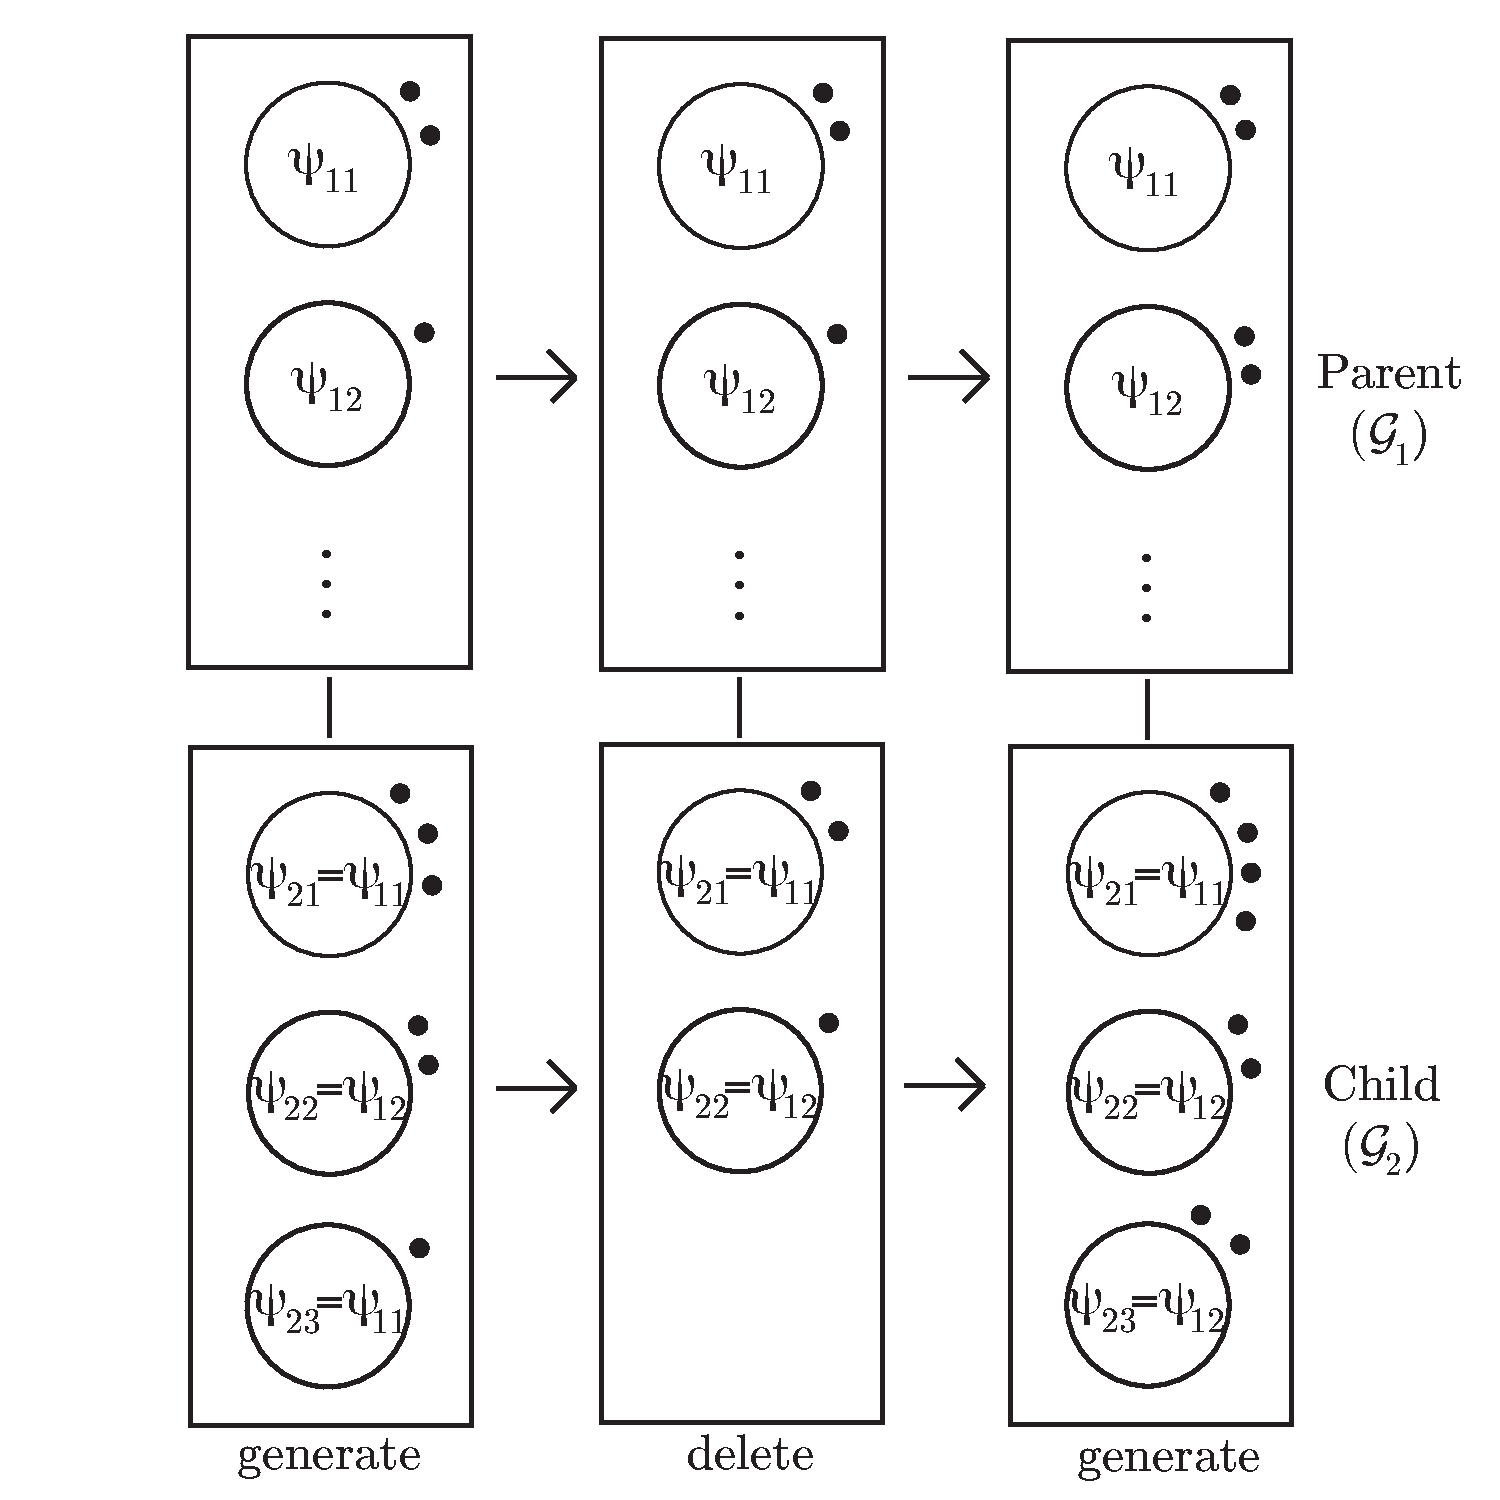
\includegraphics{figure2.pdf}} 
		\caption{Depiction of dependent hierarchical Pitman-Yor process in Chinese restaurant franchise representation}
		\label{figVHPY}
	\end{center} 
\end{figure} 

Figure~\ref{figVHPY} shows a sample from the model given in Eqn.~\ref{fig:dhpyp} generated using the procedure described in this section. The middle column of restaurants show the restaurant configurations after a deletion step.  Note the configuration of the parent restaurant does not change even though one of the tables in the child restaurant has been removed.  The restaurant configurations in the third column show the resulting seating arrangement after the sample $\{ \theta_j^2 \}_{j = 1}^5$ was generated.  Here, a customer was added to the the parent restaurant in order to generate the parameter $\psi_{12}$  given to the third table in the child restaurant.

Extending the generative procedure to draw samples from dependent HPYP's of the type
%
\begin{eqnarray}
\G_1^t | d_1, c_1, \G_0  &\sim& \PY(d_1,d_2,\G_0)  \label{fig:vhpyp2}\\
\G_2^t | d_2, c_2, \G_1^t &\sim& \PY(d_2, c_2, \G_1^t),  \hspace{.5cm} t = 1,\dots, T \nonumber \\
\theta^t_i | \G_2^t &\sim& \G_2^t, \hspace{2.28cm} i = 1, \dots, N_t \nonumber
\end{eqnarray}
%
can be done. Dependence is induced between the $\G_1^t$'s by using the deletion scheme in the parent restaurants.  In order to produce a sample from the model described by Eqn.~\ref{fig:vhpyp2} the configuration of the child restaurants must also be altered.  If we assume independence of the $\G_2^t$'s then the appropriate action is to delete all customers in the child restaurant between time steps. This is the action we are going to take. Without the assumption of independence the extension is not straightforward. It is likely that such a process exists, but we do not develop it in this paper.

While the theory developed from this point forward is applicable to all HPYP models we restrict our attention to the SM model.  This is because we are specifically interested in using the deletion process to control the memory complexity of inference in the SM.

\subsection{Constant memory}
The deletion mechanism used to define the dependent HPYP can alternatively be viewed as a way to limit the space complexity required to estimate the SM.  As noted earlier, the number of instantiated restaurants is the limiting factor regarding memory usage.  For this discussion we will therefore consider a single instantiated restaurant as a unit of memory. For the deletion scheme to limit the amount of memory used in the SM, we must be able to limit the number of instantiated restaurants.

The number of instantiated restaurants can be limited using the deletion scheme developed for dependent HPYP's. Memory savings can be achieved by deleting all the customers in a leaf restaurant since leaf restaurants without people do not need to be represented. We call a restaurant a leaf restaurant if all restaurants descended from it are empty. Nodes corresponding to leaf restaurants are shaded in Fig.~\ref{figprefixtree}.

The theory developed in Section~\ref{sec:dpyp} aids in understanding the implied dependencies that arise from deleting customers in leaf restaurants. For example, in Fig.~\ref{figprefixtree} consider what would happen if we deleted all the customers in the restaurant labeled $\G_{pa}$. Let $\G^t_{pa} = \G_{pa}$.  Implicit in this deletion is the assumption that the distribution over symbols following the context $pa$ in the sequence prior to the deletion step, $G_{pa}^t$  is, conditioned on  $\G_a$, independent of the distribution $\G_{pa}^{t+1}$ after the deletion at time $t$.

%To facilitate further discussion we will introduce a more general notation.  We will say the vector $\bf{P}$ is a path if each element is a restaurant and each restaurant is a child of the previous entry.  We will define the subtree of a restaurant as the set of all restaurants descended from it.  Finally, we say the subtree of restaurant $R$ at $t$ and $t+1$ are independent if the distributions corresponding to the restaurants of the subtree at $t$ and $t+1$ are independent conditioned by the distribution associated with restaurant $R$.

Returning to the SM model and the deletion of leaf resaurants, we note that the parent restaurant of a leaf restaurant may not be present in the SM tree.  An example is the restaurant $\G_{pata}$ in Figure~\ref{figprefixtree}. The parent restaurant of $\G_{pata}$ is $\G_{\sigma(pata)} = \G_{ata}$.  The parent in the SM tree is $\G_{\pi(pata)} = \G_a$. 

To attain memory savings by deleting restaurant $\G_{pata}$ we must also delete all of the restaurants in the path from $\G_a$ to $\G_{pata}$.  While the restaurants on this path are not instantiated in the representation of the model, they do contain customers and their deletion is significant.  The implicit model assumption made by deleting $\G_{pata}$ is that the distributions in the subtree including and below $\G_{ta}$ before the deletion step and the same distributions after the deletion step are independent.

This is the basic framework for both bounded memory algorithms we present.  That the model can vary over time may be appropriate for very long sequences. Our deletion process requires us to assume the independence of a large number of distributions.  While this may seem troubling, a key insight is that the entire set of distributions for which we must make the independence assumption are dependent on an existing node in the tree.  Much of the information will be retained in the tree by the remaining node.

Finally, we point out that the theory behind these deletion operations holds for general hierarchical Pitman-Yor processes and thus also for finite depth n-gram style models.  In Section~\ref{results} we show some results concerning this type of model as well.
